\documentclass[11pt]{article}
\usepackage{lmodern}
\usepackage{amssymb,amsmath}
\usepackage{ifxetex,ifluatex}
%\usepackage{fixltx2e} % provides \textsubscript
\usepackage{xr} % referencing external ducument
\ifnum 0\ifxetex 1\fi\ifluatex 1\fi=0 % if pdftex
  \usepackage[T1]{fontenc}
  \usepackage[utf8]{inputenc}
\else % if luatex or xelatex
  \ifxetex
    \usepackage{mathspec}
  \else
    \usepackage{fontspec}
  \fi
  \defaultfontfeatures{Ligatures=TeX,Scale=MatchLowercase}
\fi
% use upquote if available, for straight quotes in verbatim environments
\IfFileExists{upquote.sty}{\usepackage{upquote}}{}
% use microtype if available
\IfFileExists{microtype.sty}{%
\usepackage{microtype}
\UseMicrotypeSet[protrusion]{basicmath} % disable protrusion for tt fontshttps://de.overleaf.com/project/5e85b0680d0bed00011ea790
}{}
\usepackage[margin=1in]{geometry}
\usepackage{hyperref}
\hypersetup{unicode=true,
            pdftitle={Title: Limitations to the Human Neandertal Admixture dating Supplements},
            pdfauthor={Leonardo Nicola Martin Iasi (Max Planck Institute for Evolutionary Anthropology, MPI EVA), Dr.~Benjamin Marco Peter (MPI EVA, benjamin\_peter@eva.mpg.de)},
            pdfborder={0 0 0},
            breaklinks=true}
\urlstyle{same}  % don't use monospace font for urls
 
%\usepackage{natbib}
%\bibliographystyle{References/my_abbrvnat}
%\setcitestyle{authoryear,open={(},close={)}}

\usepackage{graphicx,grffile}
\makeatletter
\def\maxwidth{\ifdim\Gin@nat@width>\linewidth\linewidth\else\Gin@nat@width\fi}
\def\maxheight{\ifdim\Gin@nat@height>\textheight\textheight\else\Gin@nat@height\fi}
\makeatother
% Scale images if necessary, so that they will not overflow the page
% margins by default, and it is still possible to overwrite the defaults
% using explicit options in \includegraphics[width, height, ...]{}

\setkeys{Gin}{width=\maxwidth,height=\maxheight,keepaspectratio}
\IfFileExists{parskip.sty}{%
\usepackage{parskip}
}{% else
\setlength{\parindent}{0pt}
\setlength{\parskip}{6pt plus 2pt minus 1pt}
}
\setlength{\emergencystretch}{3em}  % prevent overfull lines
\providecommand{\tightlist}{%
  \setlength{\itemsep}{0pt}\setlength{\parskip}{0pt}}
\setcounter{secnumdepth}{0}
% Redefines (sub)paragraphs to behave more like sections
\ifx\paragraph\undefined\else
\let\oldparagraph\paragraph
\renewcommand{\paragraph}[1]{\oldparagraph{#1}\mbox{}}
\fi
\ifx\subparagraph\undefined\else
\let\oldsubparagraph\subparagraph
\renewcommand{\subparagraph}[1]{\oldsubparagraph{#1}\mbox{}}
\fi



\usepackage{setspace}
\onehalfspacing
\usepackage[left]{lineno}
\linenumbers
\usepackage[none]{hyphenat}
\usepackage{amsfonts}
\usepackage{amssymb}
\usepackage{graphicx}
\usepackage{float}
\usepackage{xcolor}

\floatplacement{figure}{H}
\begin{document}

\begin{titlepage}


    \vspace*{1cm}
        
        
    \begin{center}       
        \large
        \vspace{1cm}
        An extended admixture pulse model reveals the limits to the dating of Human-Neandertal introgression
        
       \vspace{1.0cm}
        \large
        Iasi, Leonardo N. M. \textsuperscript{1,2} and Peter , Benjamin M. \textsuperscript{1,3} \\ 
        
        \vspace{1.0cm}
            \Huge
            \textbf{Supplement Material}
    \end{center} 

            

\end{titlepage}

\section{Supplement Figures}

\begin{figure}
\centering
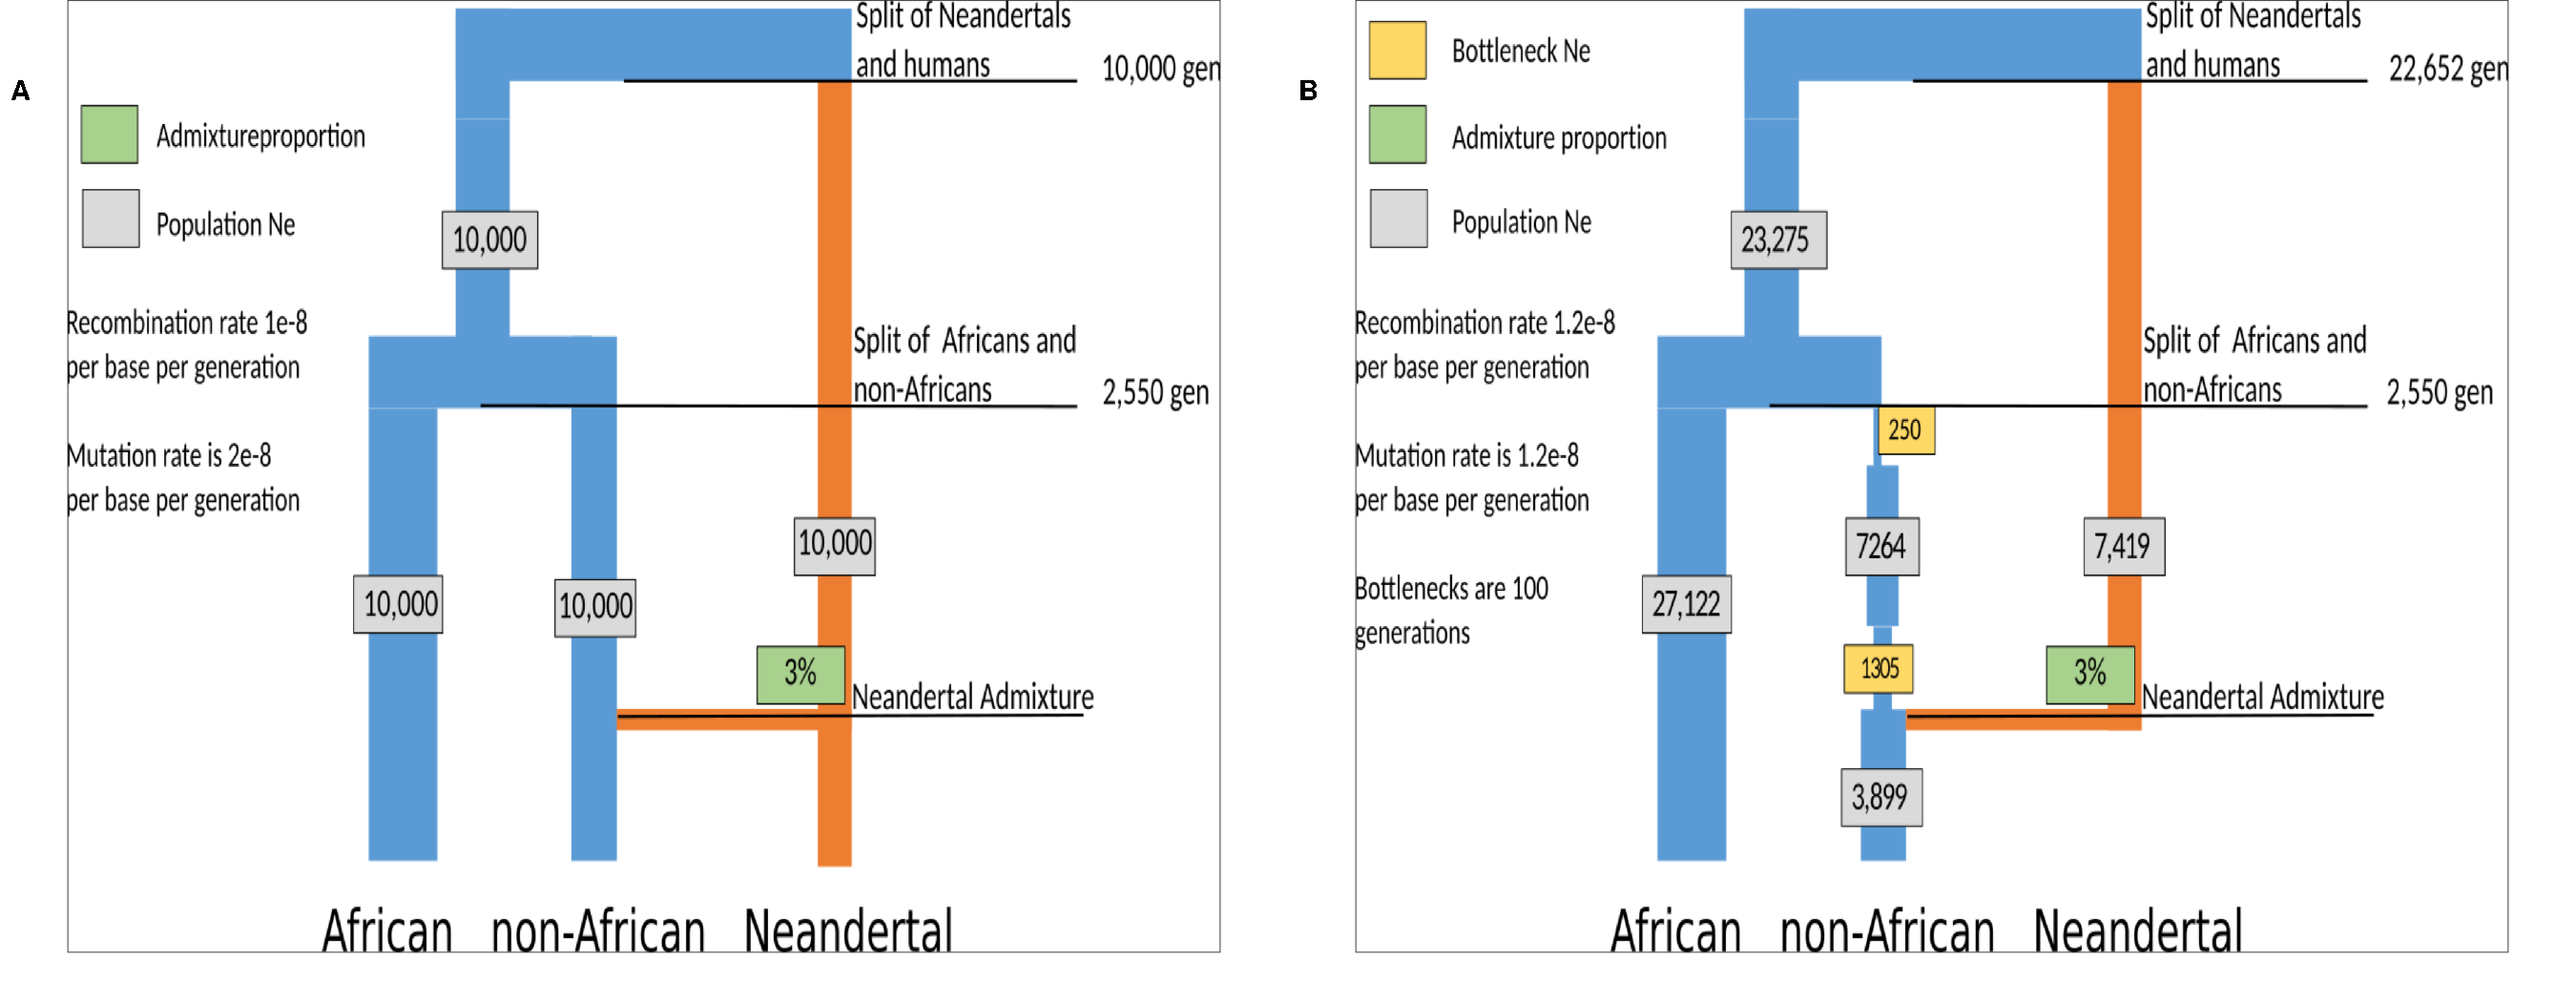
\includegraphics{Admixture_Time_Inference_Paper_Draft_files/figure-latex/Simple_and_Skov.pdf}
\caption{\label{fig:figS1} Demographic models of Neandertal introgression into non-Africans used for the simulations. A) Simple demographic model used for ALD simulations with constant population sizes. B) Complex demographic model with population size changes derived from Skov et al. 2018.}
\end{figure}

\begin{figure}
\centering
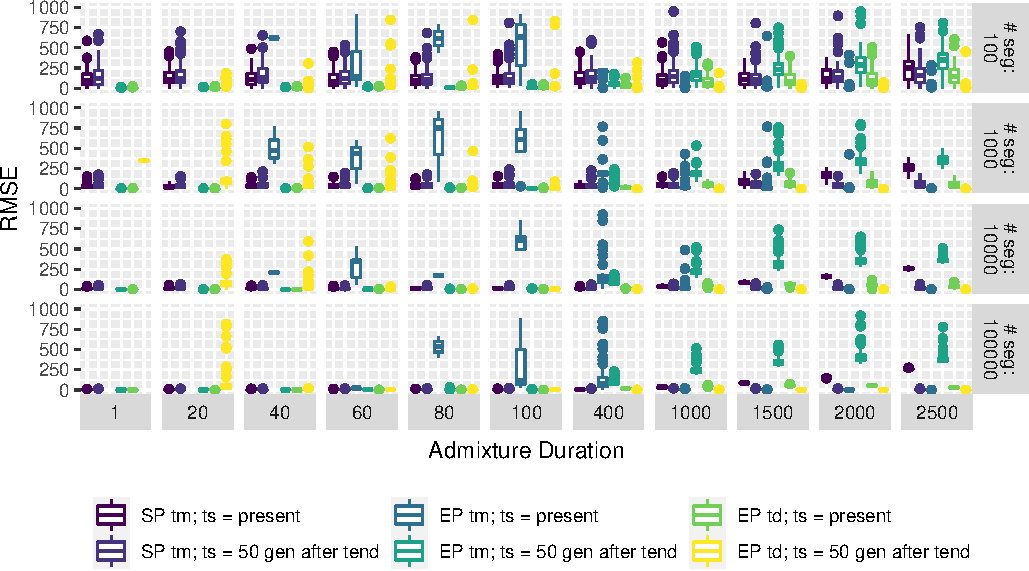
\includegraphics{ATE_Revisions_files/figure-latex/figR1_error_ests-1.pdf}
\caption{\label{fig:figR1_error_ests} Power analysis parameter estimates}
\end{figure}


\begin{figure}
\centering
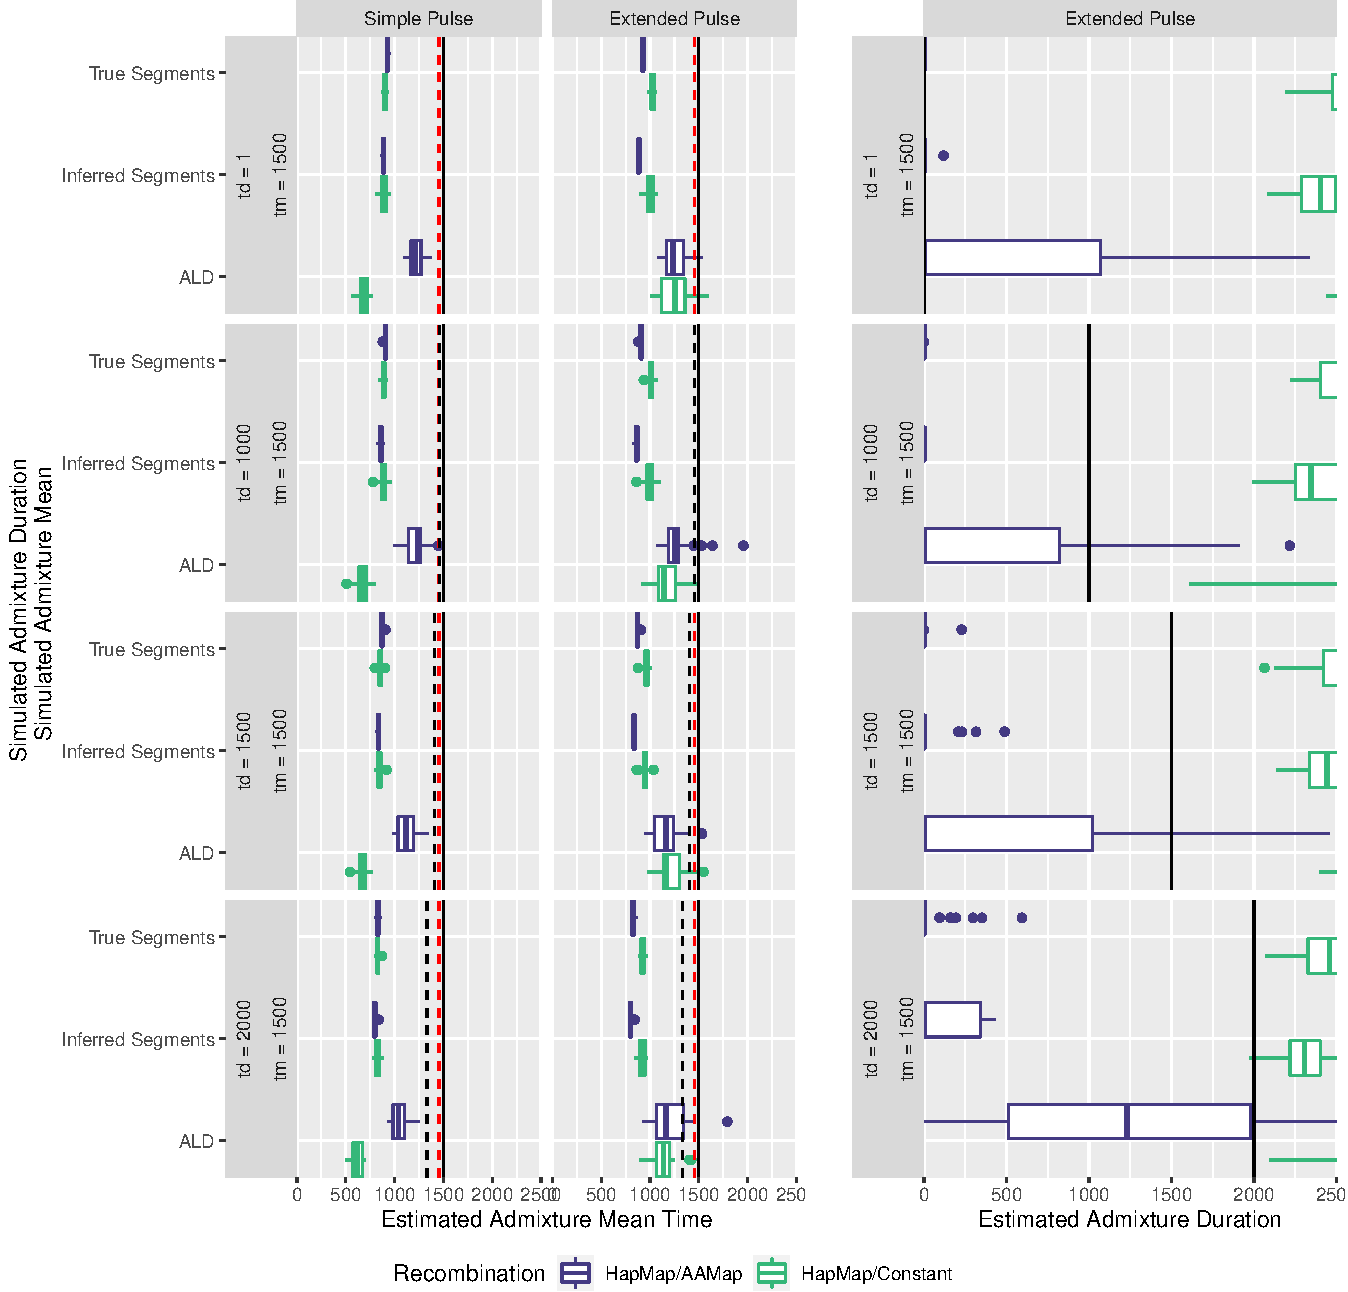
\includegraphics{ATE_Revisions_files/figure-latex/figResult2_1_Supplement-1.pdf}
\caption{\label{fig:figResult2_1_Supplements} Simple and extended pulse fitted to ALD data for different gene flow durations with mean admixture time at 1500 gnerations ago. A) Mean time estimates. B) Duration estimate.}
\end{figure}

\begin{figure}
\centering
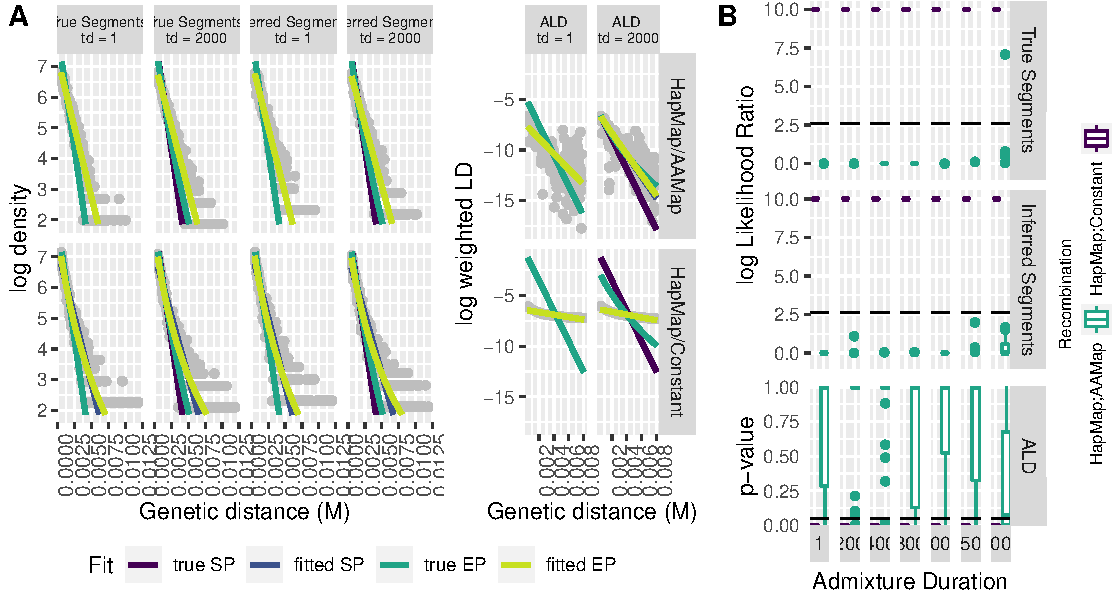
\includegraphics[width=16cm,height=18cm,keepaspectratio]{ATE_Revisions_files/figure-latex/figResult2_2and3_supplement-1.pdf}
\caption{\label{fig:fig3_2} Comparison of the fit to data between the simple and extended pulse using true and estimated parameters. }
\end{figure}

OR

\begin{figure}
\centering
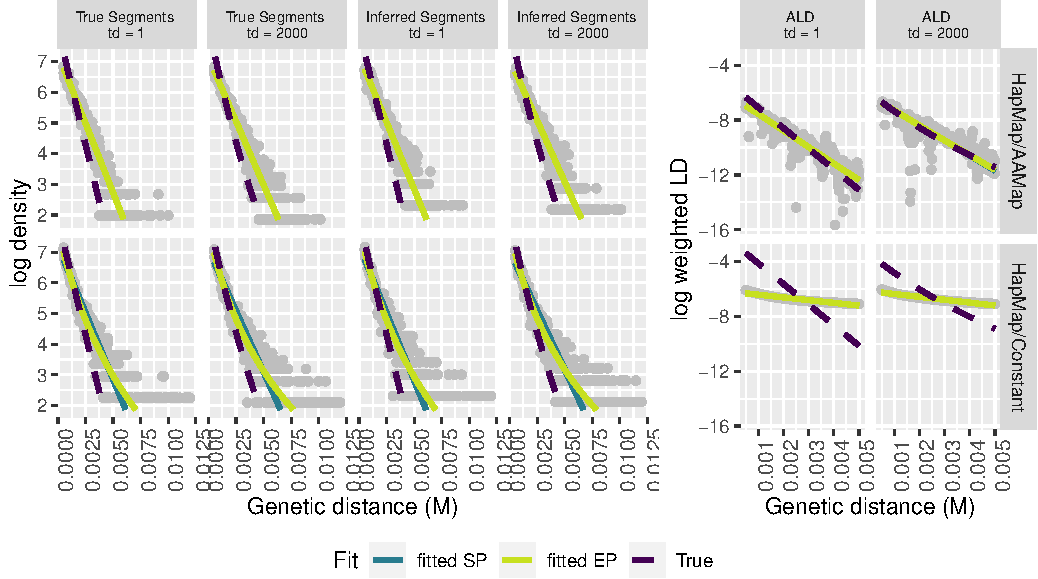
\includegraphics{ATE_Revisions_files/figure-latex/figResult2_2_Supplements-1.pdf}
\caption{\label{fig:figResult2_2_Supplements} Fit to the data}
\end{figure}

\begin{figure}
\centering
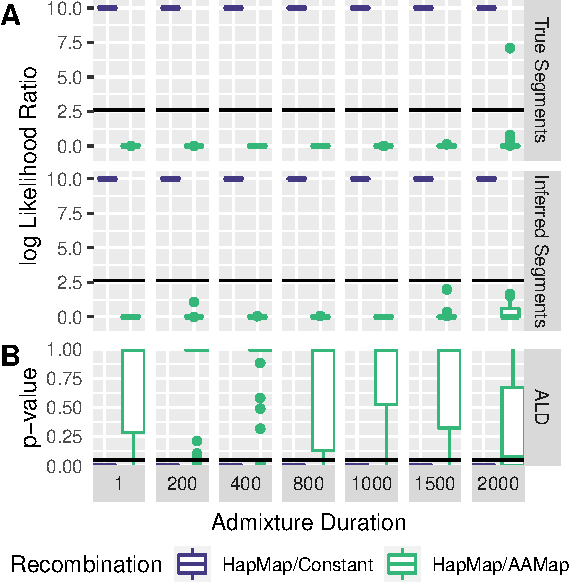
\includegraphics{ATE_Revisions_files/figure-latex/figResult2_3_supplements-1.pdf}
\caption{\label{fig:figResult2_3_Supplements} Log likelihood ratio between the simple and extended pulse fitted to ALD data for different gene flow durations with mean admixture time at 1500 gnerations ago.}
\end{figure}

\begin{figure}
\centering
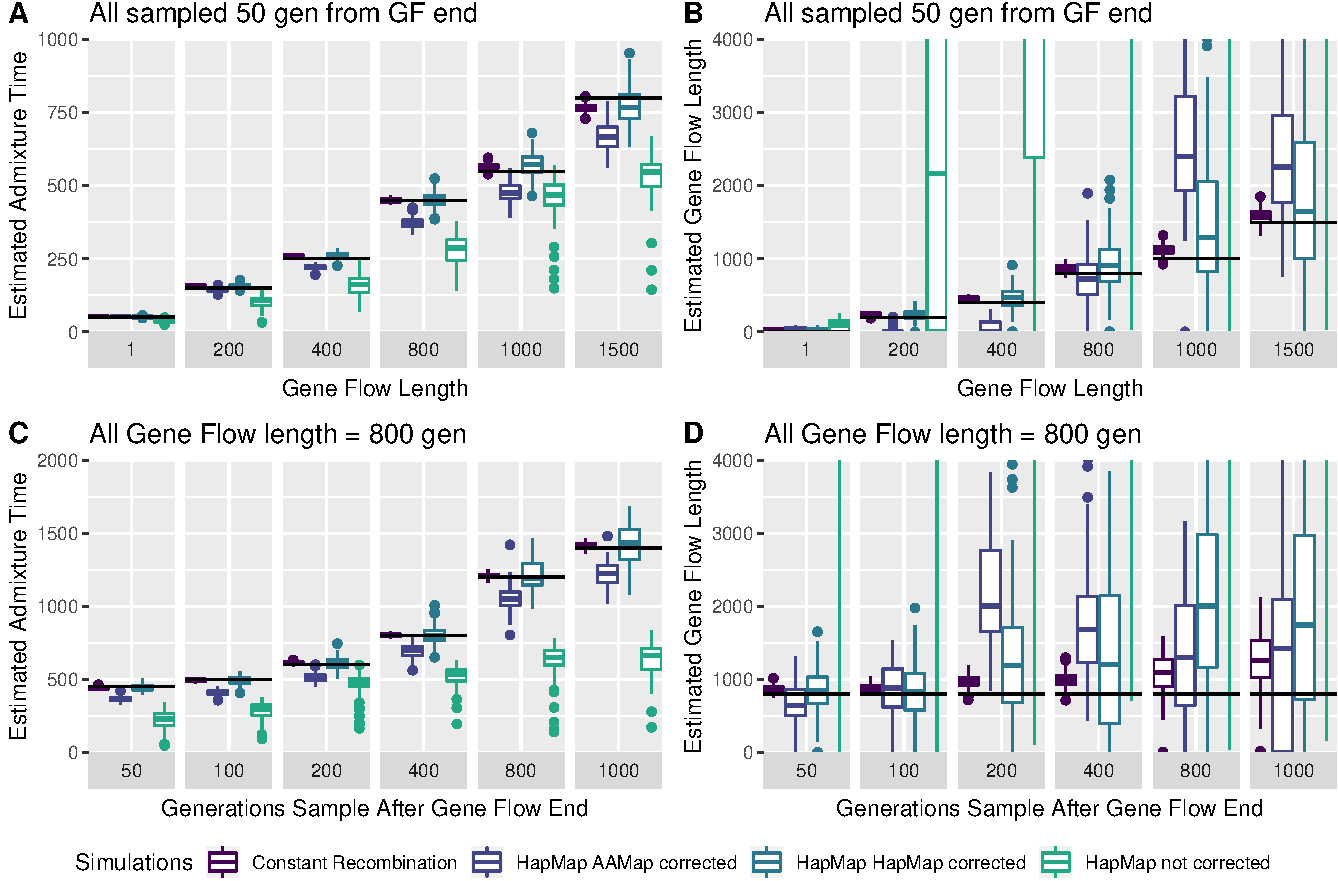
\includegraphics[width=16cm,height=18cm,keepaspectratio]{Admixture_Time_Inference_Paper_Draft_files/figure-latex/fig4-1.pdf}
\caption{\label{fig:figResult3_4_supplements} Comparison of parameter inference under the simple and extended pulse model  A) Mean time estimates $t_m$ for different gene
flow durations $t_d$ all sampled 50 generations after the gene flow ended. B)
Duration estimate $t_d$ of the same scenario C) Mean time estimates for different sampling times following 800
generations of gene flow. D) Duration estimate of the same scenario. All scenarios are simulated either under a constant recombination rate or an empirical recombination map (HapMap). Genetic distances for simulations under an empirical map are assigned by: assuming a constant rate (HapMap not corrected), using a different map (HapMap AAMap corrected) and using the same map (HapMap HapMap corrected). All times are given in generations.}
\end{figure}

\begin{figure}
\centering
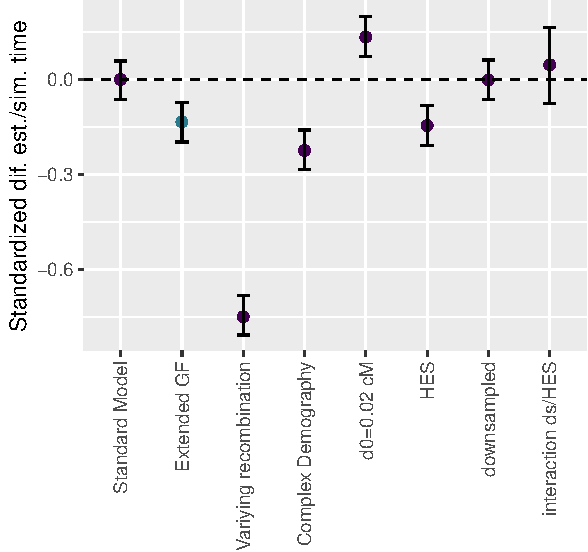
\includegraphics[width=8cm,height=16cm,keepaspectratio]{ATE_Revisions_files/figure-latex/figResult_3_supplements-1.pdf}
\caption{\label{fig:figS2_1} GLM effect size estimates and 95\% C.I. for the parameters: gene flow model (simple/extended), recombination rate (constant/varying), demography (simple/complex), minimal genetic distance (0.02/0.05 cM), SNPs used for ALD calculation (100 \% / 5 \%), ascertainment scheme (LES/HES) and additionally the interaction between ascertainment scheme and SNPs used for ALD calculation, on the standardized difference between simulated and estimated admixture time. Estimates are calculated across all possible combinations of parameters and are given as the estimate of the standard model plus the respective parameter estimate. Dotted horizontal line indicates unbiased admixture estimates.}
\end{figure}

\begin{figure}
\centering
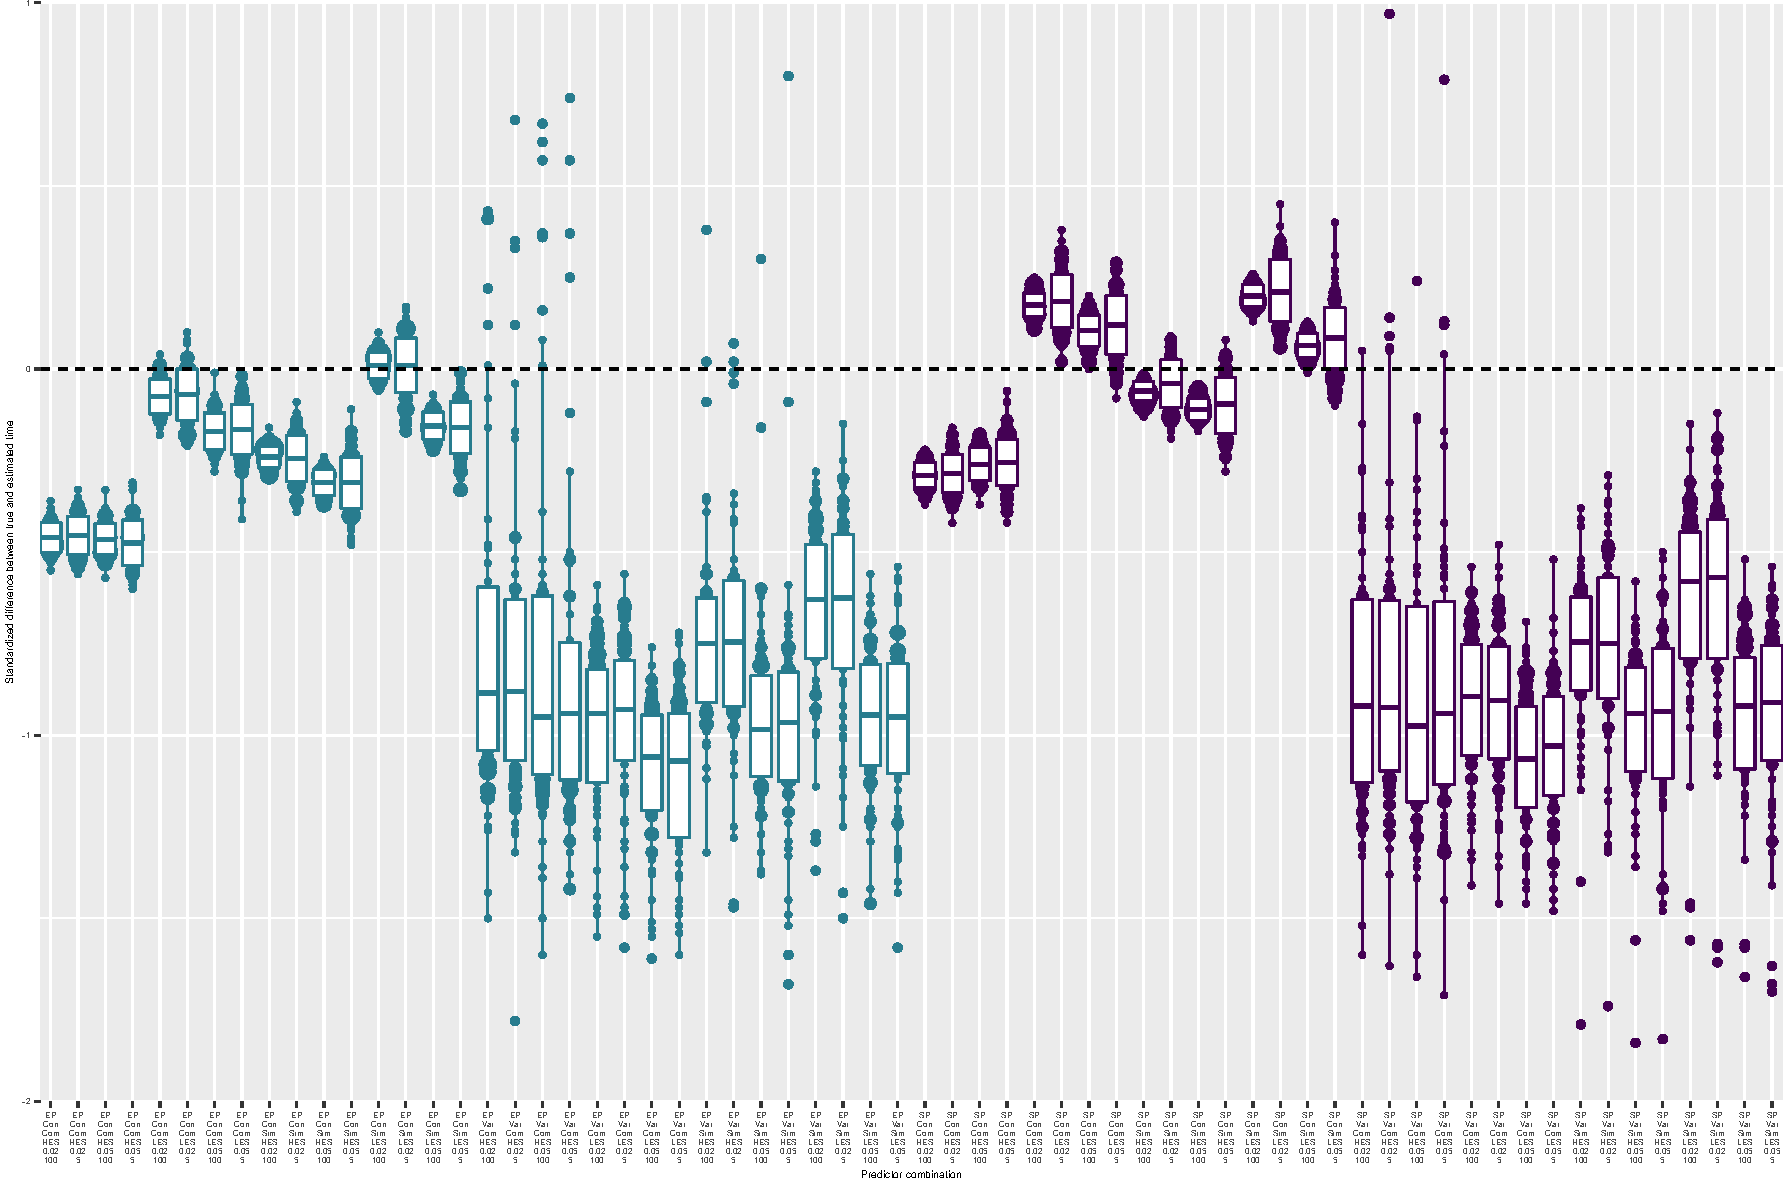
\includegraphics[width=16cm,height=18cm,keepaspectratio]{ATE_Revisions_files/figure-latex/figS2_updated-1.pdf}
\caption{\label{fig:figS2_2} Comparison of the standardized difference between true and estimated admixture time for simulations of all combinations of parameters: ascertainment scheme = LES/HES,  $d_{0}$ = 0.02/0.05 cM, demography = simple/complex, recombination = constant/variable, SNP used 100 \% / 5 \% and the gene flow model = simple/extended. Simulations under the simple pulse are indicated in purple, extended pulse in turquoise. Each simulation was repeated 100 times. Dotted horizontal line indicates no difference between true and estimated time.}
\end{figure}



\section{Supplement Tables}

\begin{table}[H]

\caption{\label{tab:tableS1_1} Mean, standard deviation, 5.5/94.5 compatibility interval of the posterior distribution for every parameter effect on the standardized difference between true and estimated admixture time.}
\centering
\begin{tabular}[t]{l|r|r|r|r|r|r}
\hline
  & mean & sd & 5.5\% & 94.5\% & n\_eff & Rhat\\
\hline
a & -0.05 & 0.03 & -0.11 & 0.01 & 2713.72 & 1\\
\cline{1-7}
bS & 0.03 & 0.02 & -0.02 & 0.07 & 4223.44 & 1\\
\cline{1-7}
bG & -0.13 & 0.02 & -0.17 & -0.08 & 3710.31 & 1\\
\cline{1-7}
bR & -0.67 & 0.02 & -0.71 & -0.62 & 4595.55 & 1\\
\cline{1-7}
bD & -0.12 & 0.02 & -0.16 & -0.07 & 4494.20 & 1\\
\cline{1-7}
bm & 0.14 & 0.02 & 0.09 & 0.18 & 4935.97 & 1\\
\cline{1-7}
bA & -0.07 & 0.02 & -0.12 & -0.03 & 4977.04 & 1\\
\cline{1-7}
sigma & 0.94 & 0.01 & 0.92 & 0.95 & 6455.01 & 1\\
\hline
\end{tabular}
\end{table}

\begin{table}[H]

\caption{\label{tab:tableS1_1}\label{tab:tableS1} Mean, standart deviation, 5.5/94.5 compatibility interval of the posterior distribution for every parameter effect on the standardized difference between true and estimated admixture time.}
\centering
\begin{tabular}[t]{l|r|r|r|r|r|r}
\hline
  & mean & sd & 5.5\% & 94.5\% & n\_eff & Rhat\\
\hline
a & -0.01 & 0.03 & -0.07 & 0.05 & 2168.04 & 1\\
\cline{1-7}
bd & 0.02 & 0.02 & -0.02 & 0.07 & 4011.95 & 1\\
\cline{1-7}
bG & -0.13 & 0.02 & -0.18 & -0.09 & 3345.76 & 1\\
\cline{1-7}
bR & -0.75 & 0.02 & -0.79 & -0.70 & 4131.16 & 1\\
\cline{1-7}
bD & -0.22 & 0.02 & -0.27 & -0.18 & 3651.09 & 1\\
\cline{1-7}
bm & 0.13 & 0.02 & 0.09 & 0.18 & 3809.54 & 1\\
\cline{1-7}
bA & -0.12 & 0.02 & -0.17 & -0.07 & 3556.78 & 1\\
\cline{1-7}
sigma & 0.91 & 0.01 & 0.90 & 0.93 & 5418.41 & 1\\
\hline
\end{tabular}
\end{table}

\begin{table}[H]

\caption{\label{tab:tableS1_2}\label{tab:tableS1} Mean, standart deviation, 5.5/94.5 compatibility interval of the posterior distribution for every parameter effect on the standardized difference between true and estimated admixture time.}
\centering
\begin{tabular}[t]{l|r|r|r|r|r|r}
\hline
  & mean & sd & 5.5\% & 94.5\% & n\_eff & Rhat\\
\hline
a & 0.00 & 0.03 & -0.06 & 0.06 & 1823.65 & 1\\
\cline{1-7}
bdA & 0.05 & 0.04 & -0.04 & 0.14 & 2049.11 & 1\\
\cline{1-7}
bd & 0.00 & 0.03 & -0.06 & 0.06 & 2156.79 & 1\\
\cline{1-7}
bG & -0.13 & 0.02 & -0.18 & -0.09 & 2865.05 & 1\\
\cline{1-7}
bR & -0.75 & 0.02 & -0.79 & -0.71 & 3405.94 & 1\\
\cline{1-7}
bD & -0.22 & 0.02 & -0.27 & -0.18 & 3128.70 & 1\\
\cline{1-7}
bm & 0.13 & 0.02 & 0.09 & 0.18 & 3850.41 & 1\\
\cline{1-7}
bA & -0.15 & 0.03 & -0.21 & -0.08 & 2335.16 & 1\\
\cline{1-7}
sigma & 0.91 & 0.01 & 0.90 & 0.93 & 3894.49 & 1\\
\hline
\end{tabular}
\end{table}

\begin{table}[H]

\caption{\label{tab:tableS2_2}\label{tab:tableS2} AIC and RSS for the fit to Neandertal data}
\centering
\begin{tabular}[t]{l|r|r}
\hline
Model & AIC & RSS\\
\hline
Simple Pulse & -44845.31 & 4.33e-05\\
\hline
Extended Pulse (td=1) & -44845.31 & 4.33e-05\\
\hline
Extended Pulse (td=100) & -44846.42 & 4.33e-05\\
\hline
Extended Pulse (td=200) & -44849.73 & 4.32e-05\\
\hline
Extended Pulse (td=400) & -44862.90 & 4.30e-05\\
\hline
Extended Pulse (td=800) & -44914.33 & 4.23e-05\\
\hline
Extended Pulse (td=1000) & -44951.47 & 4.18e-05\\
\hline
Extended Pulse (td=1500) & -45069.45 & 4.01e-05\\
\hline
Extended Pulse (td=2000) & -45200.02 & 3.84e-05\\
\hline
Extended Pulse (td=2500) & -45294.46 & 3.72e-05\\
\hline
\end{tabular}
\end{table}

\end{document}